\subsection{Gasgefüllter Ionisationsdetektor}
Im letzten Schritt treffen die verbliebenen Ionen in den Ionisationsdetektor ein, der mit Isobutan ($C_{4}H_{10}$) gefüllt ist.
Auch hier verlieren die Ionen wieder Energie beim durchqueren des Mediums.
Dadurch ionisieren sie das Isobutan.
Die entstandenen freien Ladungsträger werden durch das elektrische Feld abgesaugt und führen zu einem detektierbaren Strom.
Die Dichte des Isobutan wurde mit der thermischen Zustandsgleichung idealer Gase abgeschätzt:
\begin{gather}
    \rho = \frac{p \cdot m}{k_{B} \cdot T}
\end{gather}
Wobei $k_{B}$ die Boltzmann-Konstante ist.
Der Druck $p$ war angegeben mit \SI{31.0e-3}{\bar}, die Temperatur $T$ mit \SI{21.0}{\degreeCelsius} und die Masse eines Isobutan-Moleküls $m$ ist etwa \SI{58}{\atomicmassunit}.
Damit ergibt sich eine Dichte von \SI{7e-5}{\gram\per\cubic\centi\metre}.
Mithilfe von SRIM lassen sich nun wieder die Abbremsungen ermitteln.
Da diese selbst Energieabhängig sind gelten einzelne Werte nur für kleine Energieänderungen.
Trotzdem können wir mit ihnen eine Abschätzung der Eindringtiefe der Ionen in den Detektor vornehmen, zu finden in Tabelle \ref{Auswertung_tab_Gasdetektor_Eindringtiefen}.
\begin{center}
  \begin{tabular}{|c|c|c|c|}
    \hline
    Ion (nach Folie) & Energie nach Folie & $\frac{\Delta E}{\Delta x}$ (zu Beginn) & Eindringtiefe im Detektor \\
    \hline
    \multirow{4}*{$^{10}\text{Be}^{4+}$} & \SI{6.2}{\mega\electronvolt}  & \SI{0.0464}{\mega\electronvolt\per\milli\metre} & \SI{134}{\milli\metre}  \\
                                         & \SI{11.7}{\mega\electronvolt} & \SI{0.0339}{\mega\electronvolt\per\milli\metre} & \SI{344}{\milli\metre}  \\
                                         & \SI{17.1}{\mega\electronvolt} & \SI{0.0262}{\mega\electronvolt\per\milli\metre} & \SI{650}{\milli\metre}  \\
                                         & \SI{22.4}{\mega\electronvolt} & \SI{0.0214}{\mega\electronvolt\per\milli\metre} & \SI{1047}{\milli\metre} \\
    \hline
    \multirow{4}*{$^{10}\text{B}^{4+}$}  & \SI{5.8}{\mega\electronvolt}  & \SI{0.0641}{\mega\electronvolt\per\milli\metre} & \SI{91}{\milli\metre}   \\
                                         & \SI{11.3}{\mega\electronvolt} & \SI{0.0495}{\mega\electronvolt\per\milli\metre} & \SI{228}{\milli\metre}  \\
                                         & \SI{16.7}{\mega\electronvolt} & \SI{0.0391}{\mega\electronvolt\per\milli\metre} & \SI{427}{\milli\metre}  \\
                                         & \SI{22.1}{\mega\electronvolt} & \SI{0.0322}{\mega\electronvolt\per\milli\metre} & \SI{686}{\milli\metre}  \\
    \hline
  \end{tabular}
  \captionof{table}{Eindringtiefe der Ionen in den Detektor. Bor ist mit aufgenommen um zu untersuchen ob das Isobar vollständig beseitigt werden konnte. Da der Detektor nur eine Länge von etwa \SI{30}{\centi\metre} hat würden einige Ionen den Detektor wieder verlassen. Da der Energieverlust als konstant angenommen wurde überschätzt diese Rechnung die Eindringtiefe.}
  \label{Auswertung_tab_Gasdetektor_Eindringtiefen}
\end{center}
Mit den Eindringtiefen wird klar, dass $^{10}\text{Be}$, welches nach der Mitte des Tandems einen Ladungszustand von $3+$ oder mehr hatte durch den Detektor durchfliegen würde.
Es bietet sich daher für die Messung an $^{10}\text{Be}^{2+}$ Ionen auszuwählen (Die Magneten und den ESA darauf einstellen).
Dies wurde in den aufgenommenen Spektren getan.
In Abb. \ref{Auswertung_Gasdetektor_2DSpektren} sind diese für verschiedene Proben zu finden.
\begin{figure}[h]
    \begin{subfigure}{0.95\textwidth}
        \centering
        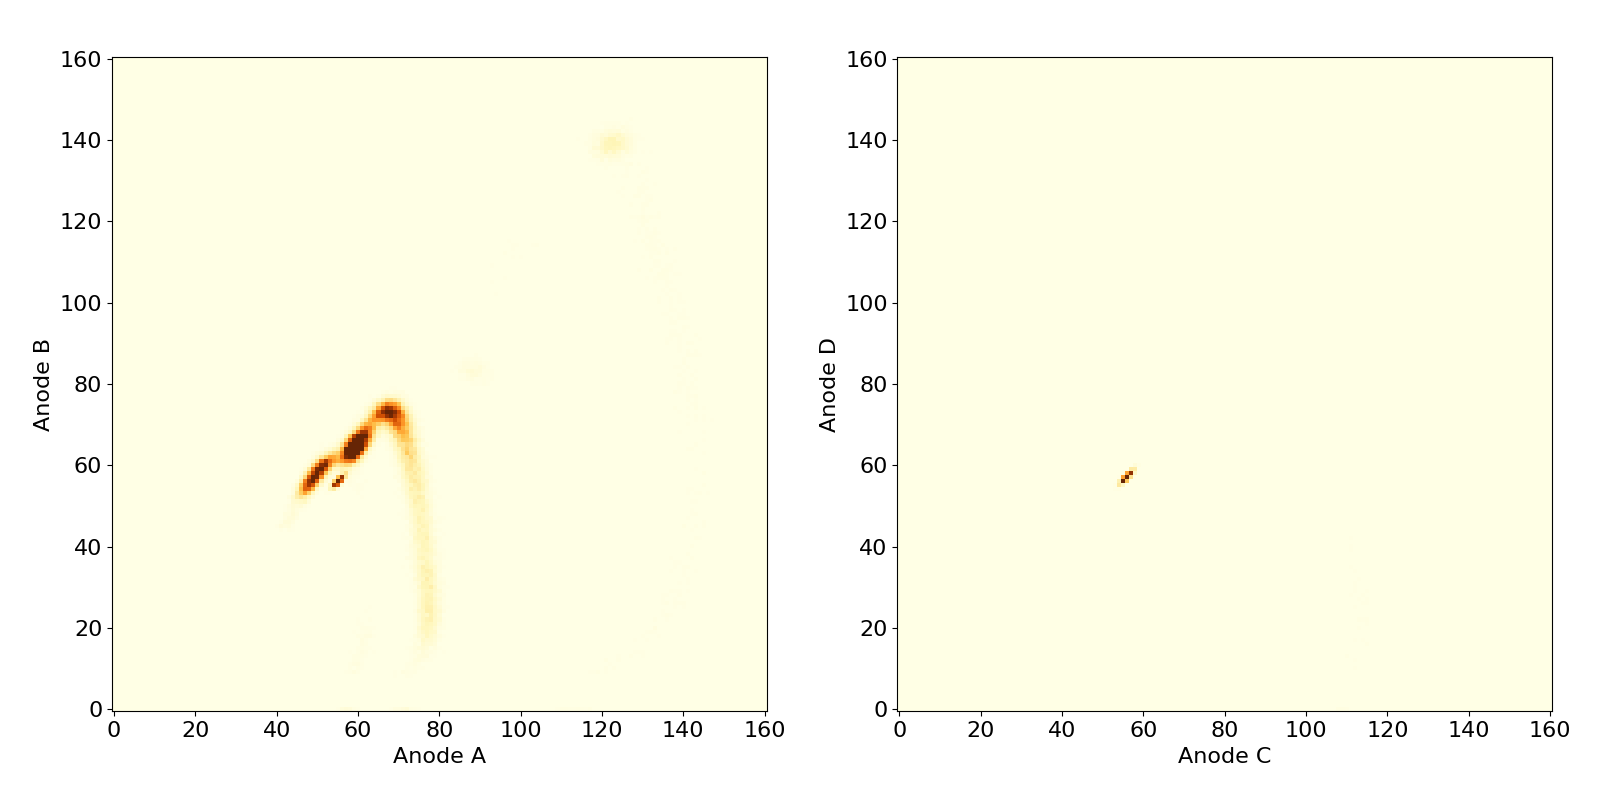
\includegraphics[width=0.95\linewidth]{Pictures/Gasdetektor/Gasdetektor_2DSpektrum_3.png}
        \caption{Ohne Probe, live-Zeit von $t_{\text{live}} = \SI{1245}{\second}$}
    \end{subfigure}
    \begin{subfigure}{0.95\textwidth}
        \centering
        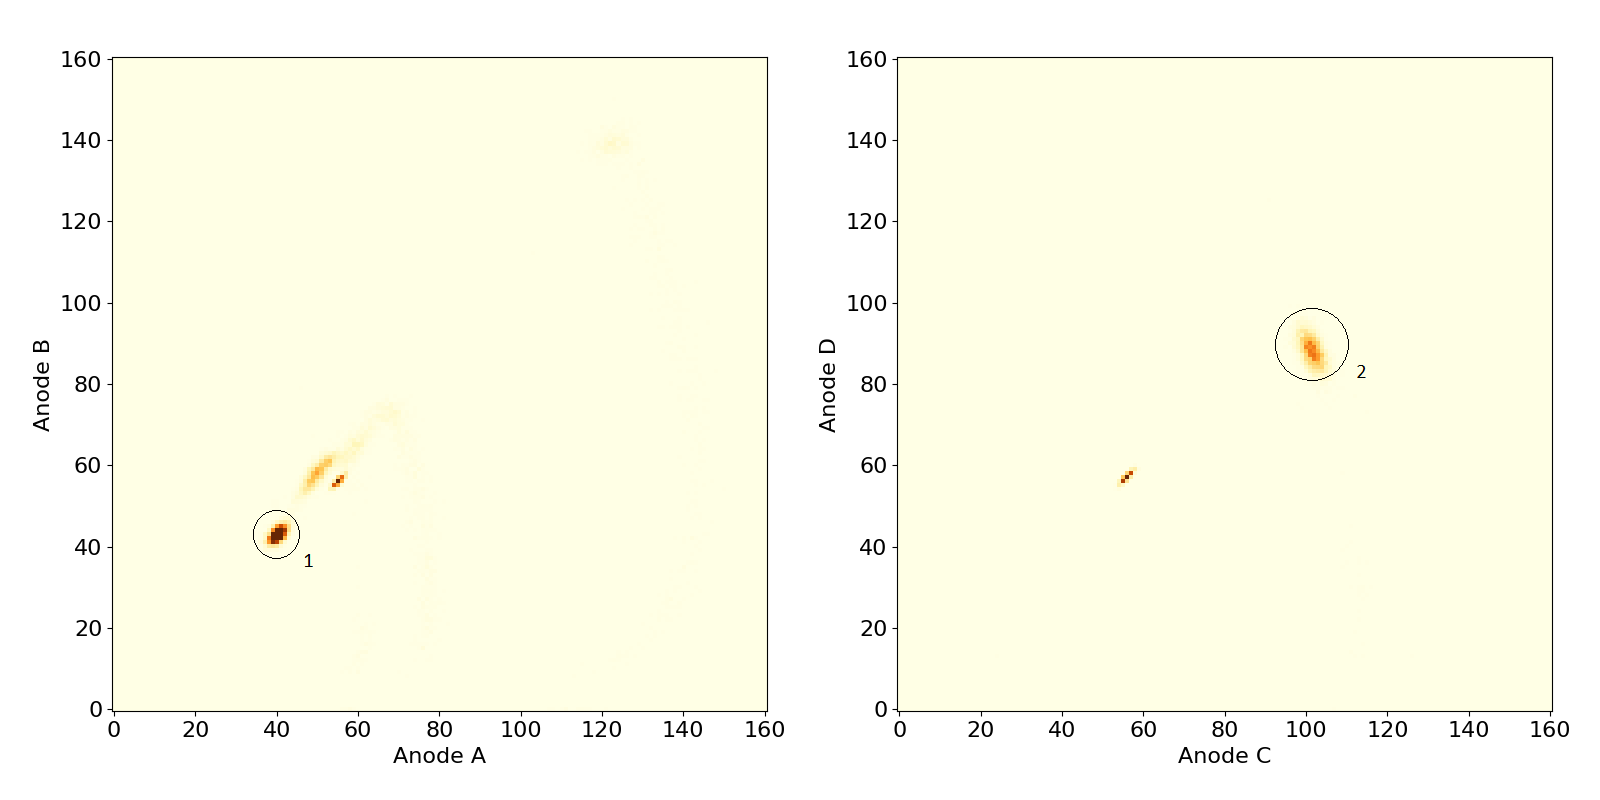
\includegraphics[width=0.95\linewidth]{Pictures/Gasdetektor/Gasdetektor_2DSpektrum_22.png}
        \caption{BeO-Probe, live-Zeit von $t_{\text{live}} = \SI{474}{\second}$}
    \end{subfigure}
    \begin{subfigure}{0.95\textwidth}
        \centering
        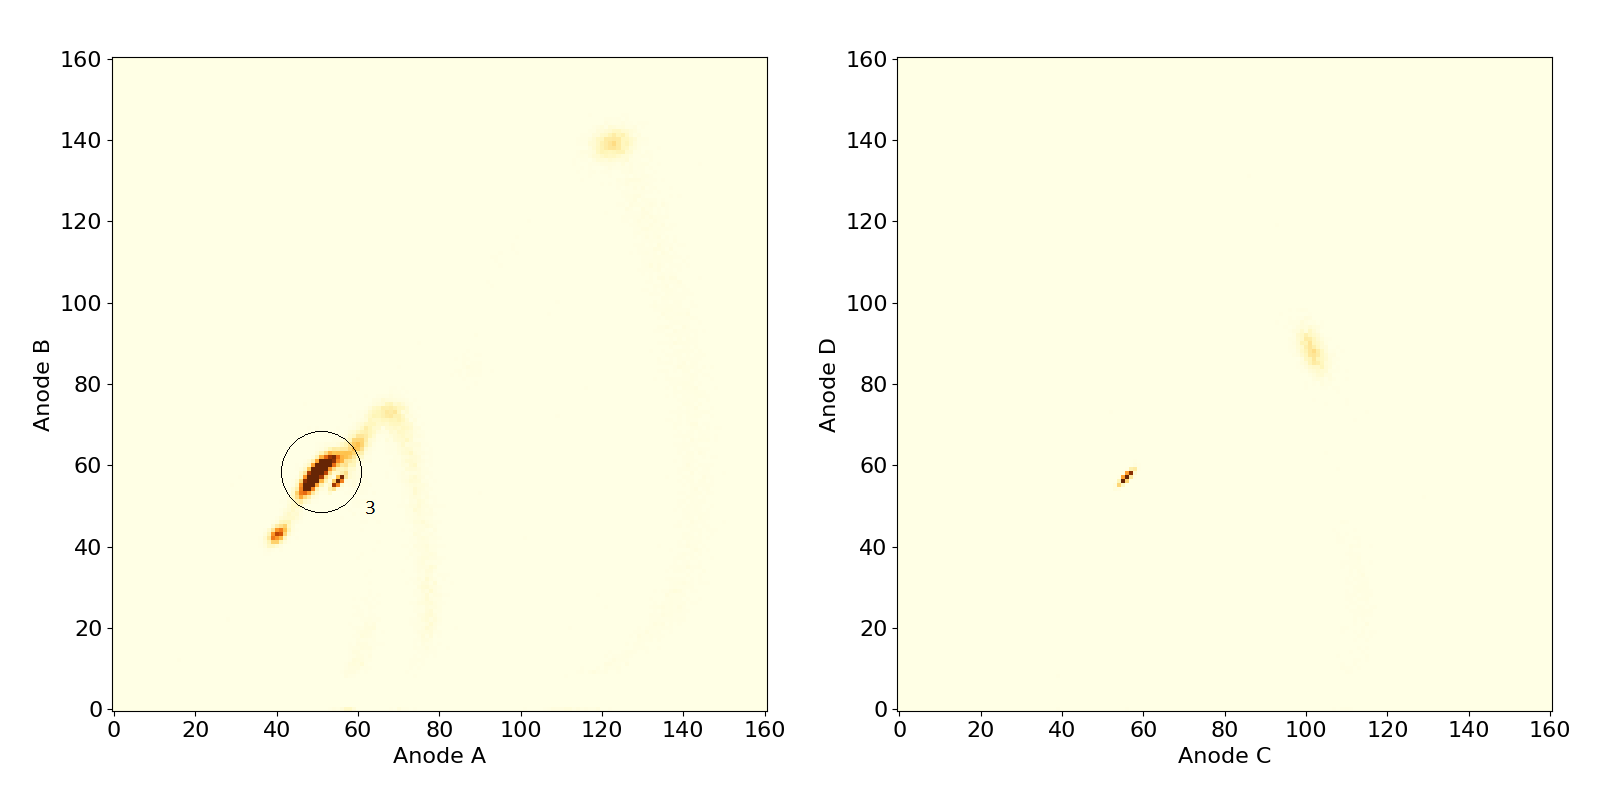
\includegraphics[width=0.95\linewidth]{Pictures/Gasdetektor/Gasdetektor_2DSpektrum_19.png}
        \caption{Unbekannte Probe, live-Zeit von $t_{\text{live}} = \SI{845}{\second}$}
    \end{subfigure}
    \caption{2D-Spektren der Anoden in der Gasionisationskammer. Markiert sind einige \glqq Fingerabdrücke\grqq{} von Ionen. Je mehr Rot/Braun ein Pixel ist, desto mehr Ereignisse wurden in diesem Punkt registriert. Die Achsen sind mit den Kanälen des ADC beschriftet. Diese laufen eigentlich bis \num{255}, jedoch gibt es in den höheren Bereichen keine Ereignisse.}
    \label{Auswertung_Gasdetektor_2DSpektren}
\end{figure}
In den Spektren ist zu erkennen, dass es für die Kombination Anode A und B, sowie für die Kombination C und D im wesentlichen jeweils zwei Stellen gibt, die von Null verschieden sind.
Diese werden durch die Spektren der BeO-Probe und der unbekannten Probe ganz gut voneinander getrennt.
Dies wird vor allem ersichtlich, wenn man diese Proben in einem Diagramm vereint, wie in \ref{Auswertung_Bild_Gasdetektor_2DSpektren_BeO_unbekannt_relativ} geschehen.
\begin{figure}[h]
	\centering
    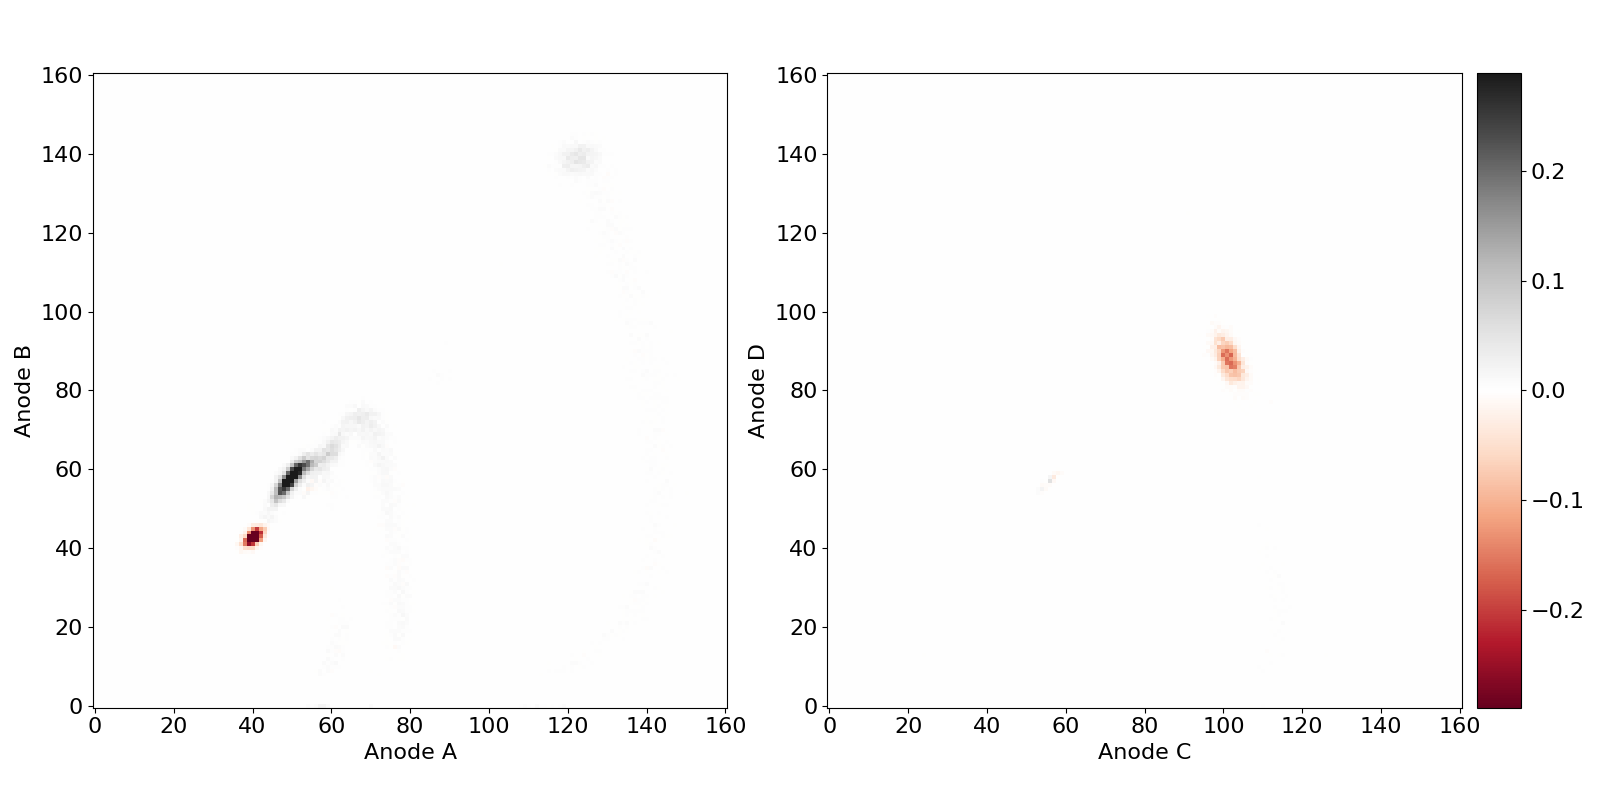
\includegraphics[width=0.95\textwidth]{Pictures/Gasdetektor/Gasdetektor_2DSpektrum_19_relativ_zu_22.png}
	\caption{Plot der Spektren der BeO-Probe und der unbekannten Probe. Gezeigt ist die Differenz der Spektren der Proben, wobei jeder Pixel jedes Spektrums durch die live-Zeit des Detektors während der jeweiligen Messung geteilt wurde. Positive Werte (schwarz) stammen praktisch von der unbekannten Probe, negative (rot) von der BeO-Probe.}
	\label{Auswertung_Bild_Gasdetektor_2DSpektren_BeO_unbekannt_relativ}
\end{figure}
Spätestens damit wird klar, dass es sich in dem Bereich um zwei verschiedene Ionen handeln muss.
Der mit $1$ und der mit $2$ markierte Bereich gehört zum $^{10}\text{Be}$.
Den mit $3$ markierten Bereich (bis auf die kleine Insel unten rechts von dem Großteil) ordnen wir $^{10}\text{B}$ zu.
Eigentlich sollte dieses herausgefiltert sein, eine Begründung für die Zuordnung folgt gleich.
Zuerst möchten wir die Aufmerksamkeit auf den kleinen Fleck in jedem der 3 Spektren lenken, der immer etwa bei den Kanälen $(60, 60)$ auftritt.
Da dieser Fleck immer an der selben Stelle auftritt ist darauf zu schließen, dass es sich um ein oder einige sehr Energiereiche Ionen handelt.

Um die restlichen Flecken näher zu untersuchen sind in Abb. \ref{Auswertung_Gasdetektor_TRIM_sims} und \ref{Auswertung_Gasdetektor_TRIM_sim_Bor} einige TRIM-Simulationen vorgenommen worden.
\begin{figure}[h]
    \begin{subfigure}{0.45\textwidth}
        \centering
        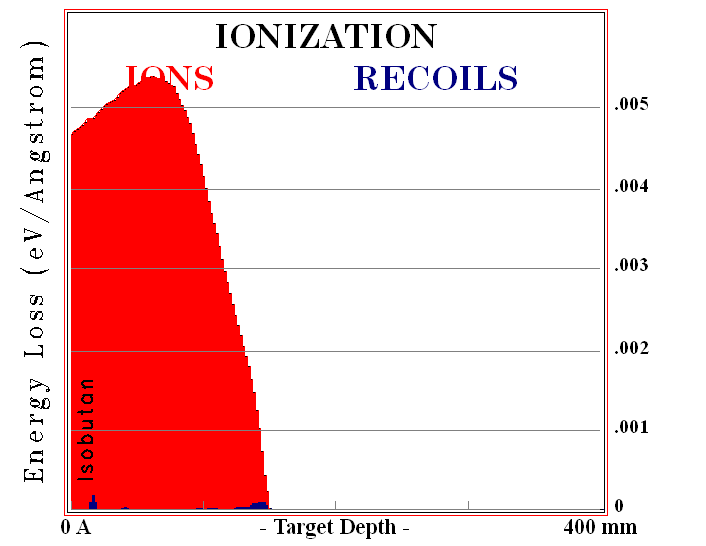
\includegraphics[width=0.95\linewidth]{Pictures/TRIM_Ionisierung_10Be_in_Isobutan_vorher_1+.png}
        \caption{$E_{\text{Ion, Start}} = \SI{6.2}{\mega\electronvolt}$ (vor Folie $^{10}\text{Be}^{1+}$)}
        \label{Auswertung_Gasdetektor_TRIM_sims_a}
    \end{subfigure} \qquad
    \begin{subfigure}{0.45\textwidth}
        \centering
        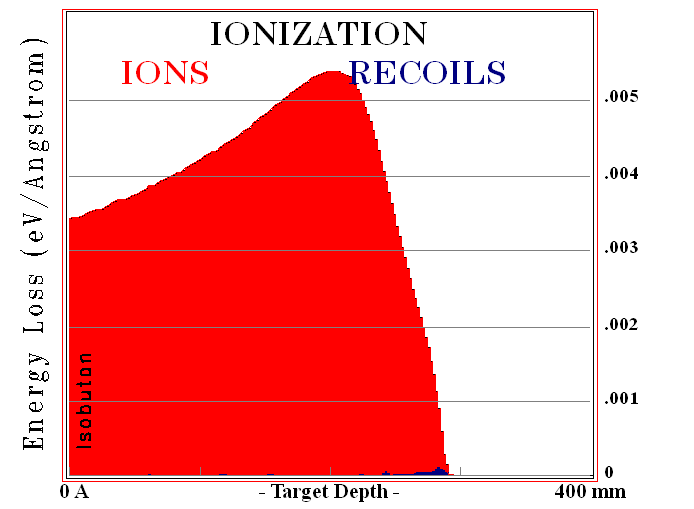
\includegraphics[width=0.95\linewidth]{Pictures/TRIM_Ionisierung_10Be_in_Isobutan_vorher_2+.png}
        \caption{$E_{\text{Ion, Start}} = \SI{11.7}{\mega\electronvolt}$ (vor Folie $^{10}\text{Be}^{2+}$)}
        \label{Auswertung_Gasdetektor_TRIM_sims_b}
    \end{subfigure} \\
    \begin{subfigure}{0.45\textwidth}
        \centering
        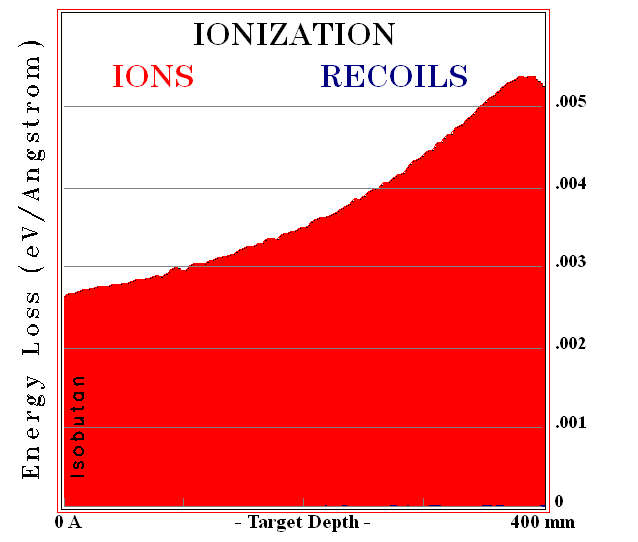
\includegraphics[width=0.95\linewidth]{Pictures/TRIM_Ionisierung_10Be_in_Isobutan_vorher_3+.png}
        \caption{$E_{\text{Ion, Start}} = \SI{17.1}{\mega\electronvolt}$ (vor Folie $^{10}\text{Be}^{3+}$)}
        \label{Auswertung_Gasdetektor_TRIM_sims_c}
    \end{subfigure} \qquad
    \begin{subfigure}{0.45\textwidth}
        \centering
        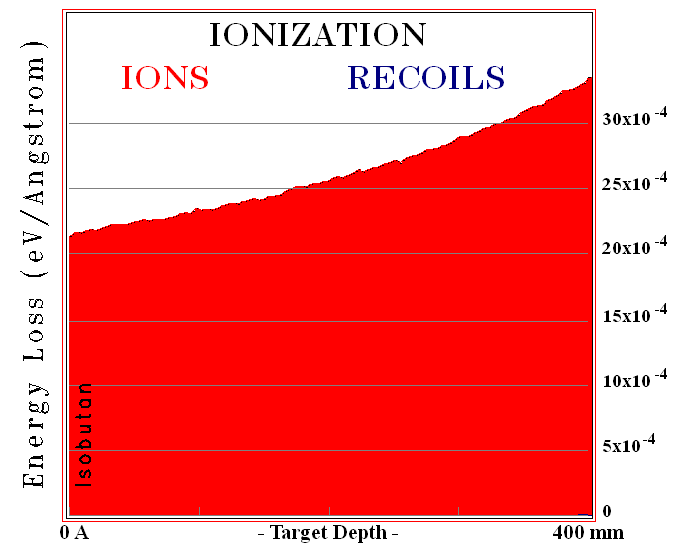
\includegraphics[width=0.95\linewidth]{Pictures/TRIM_Ionisierung_10Be_in_Isobutan_vorher_4+.png}
        \caption{$E_{\text{Ion, Start}} = \SI{22.4}{\mega\electronvolt}$ (vor Folie $^{10}\text{Be}^{4+}$)}
        \label{Auswertung_Gasdetektor_TRIM_sims_d}
    \end{subfigure}
    \caption{TRIM-Simulationen für die Ionisierung von Isobutan durch $^{10}\text{Be}$, welches mit verschiedenen Energien anfängt. Die verschiedenen Anfangsenergien sind zur Illustration der Energieabhängigkeit der Eindringtiefe. In dem Versuch können durch die Vorselektion nur Ionen mit $E_{\text{Ion, Start}} = \SI{11.7}{\mega\electronvolt}$ in den Detektor gelangen.}
    \label{Auswertung_Gasdetektor_TRIM_sims}
\end{figure}
\begin{figure}[h]
	\centering
    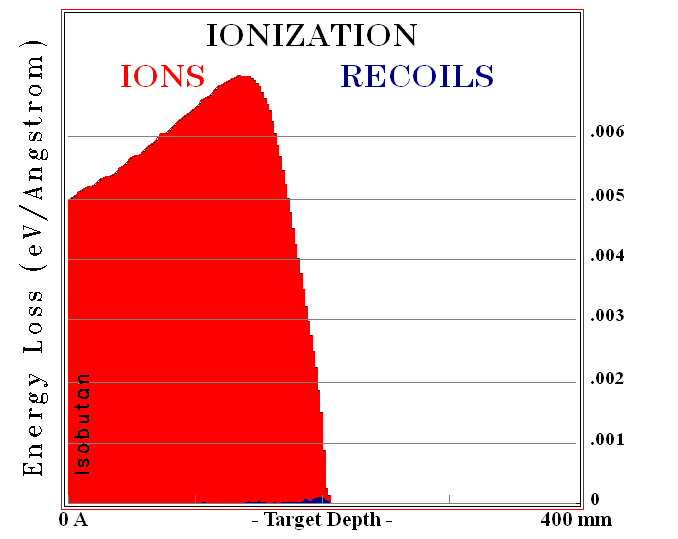
\includegraphics[width=0.45\textwidth]{Pictures/TRIM_Ionisierung_10Bor_in_Isobutan_vorher_2+.png}
	\caption{TRIM-Simulation für die Ionisierung von Isobutan durch $^{10}\text{B}$, mit Anfangsenergie $E_{\text{Ion, Start}} = \SI{11.3}{\mega\electronvolt}$ (vor Folie $^{10}\text{B}^{2+}$)}
	\label{Auswertung_Gasdetektor_TRIM_sim_Bor}
\end{figure}
Die Fläche unter den Ionisierungskurven bis zu einer bestimmten Eindringtiefe bestimmt den Ort des Ions in den 2-D-Spektren.
Es wird ersichtlich, dass Ionen, die vor der Folie $^{10}\text{Be}^{2+}$ waren (Ionisierungskurve \ref{Auswertung_Gasdetektor_TRIM_sims_b}), viel Energie im Bereich der ersten beiden Anoden, und damit im jeweils linken Spektrum am Fleck $1$ lassen.
Den Hauptteil der Energie lassen diese Ionen jedoch im Bereich zwischen \SI{100}{\milli\metre} und \SI{300}{\milli\metre}, weshalb der Fleck $2$ im rechten Spektrum bei höheren Energien liegt.
$^{10}\text{B}$ sollte eigentlich aussortiert sein, jedoch passt die Ionisierungskurve \ref{Auswertung_Gasdetektor_TRIM_sim_Bor} sehr gut zum Fleck $3$, denn er tritt nur in den linken Spektren auf.
Es lässt all seine Energie im Bereich bis \SI{200}{\milli\metre}, daher gibt es keinen Fleck in den rechten Spektren, denn dafür müsste auch auf Anode D ein Signal gemessen werden.
Außerdem hat dieser Fleck in den Spektren einen \glqq Schweif\grqq{}, was darauf schließen lässt, dass einige Ionen mit weniger Energie eintreffen (sie lassen ihre Energie vor allem im Bereich der Anode A).
DIe Ursache für all dies könnte im elektrostatischen Analysierer liegen.
Möglicherweise ist die abweichende Ablenkung durch den Geschwindigkeitsverlust in der dünnen Folie nicht genug um Bor ganz aus dem Strahl zu entfernen.
Sie reicht jedoch um die beiden Isobare im Spektrum zu unterscheiden.
Der Schweif lässt darauf schließen, das einiges von dem Bor Energie auf dem Weg zum Detektor an umliegendes Material abgibt.
Möglicherweise kollidiert es mit dem Strahlrohr und wird dann wieder vom Ionenstrahl mitgerissen.
Das würde auch erklären warum der Schweif höhere Energien im Spektrum erreicht als das Zentrum (das gebremste Bor wird nach Kollision vom schnelleren Beryllium mitgerissen).
Insgesamt lässt sich also bei der unbekannten Probe auf einen höheren $^{10}\text{B}$ Anteil schließen.
